\documentclass[journal]{IEEEtran}
\usepackage{amsmath}    % Para fórmulas matemáticas
\usepackage{amssymb}    % Para símbolos matemáticos adicionales
\usepackage{amsfonts}   % Para fuentes de matemáticas
\usepackage{graphicx}   % Para incluir imágenes
\usepackage{subcaption}
\usepackage{cite}       % Para gestionar las citas bibliográficas
\usepackage{booktabs}   % Para tablas con líneas profesionales
\usepackage{multirow}   % Para celdas de múltiples filas en tablas
\usepackage{float}      % Para mejor control de la ubicación de las figuras
\usepackage[utf8]{inputenc}
\usepackage[T1]{fontenc}
\usepackage{booktabs,siunitx,makecell,multirow,tabularx}
\usepackage[para,online,flushleft]{threeparttable}
\sisetup{
	group-separator = {\,},   
	group-minimum-digits = 4,
	output-decimal-marker = {.}
}

\title{ CO$_{2}$ classification analysis for AI models}

\author{
	\IEEEauthorblockN{Juan Felipe Gallo Rendón\IEEEauthorrefmark{1}}
	\IEEEauthorblockA{\textit{Engineering department} \\
		\textit{University of Antioquia}\\
		Medellín, Colombia}
}

\begin{document}
	\maketitle

\begin{abstract}
	This study presents a comprehensive classification analysis of artificial intelligence models based on their carbon footprint and performance metrics. A workflow was implemented, beginning with an unsupervised cluster analysis (hierarchical and k-means) to identify the intrinsic data structure, which revealed that model popularity (\texttt{downloads}, \texttt{likes}) is the primary natural segmentation factor. Subsequently, the feasibility of Linear Discriminant Analysis (LDA) was assessed through a ity diagnostic, which showed significant deviations and justified the use of a regularized variant. Finally, the performance of LDA was compared against two non-linear models—a Support Vector Machine with an RBF kernel (SVM-RBF) and Gradient Boosting (GB)—to predict a binary "fairness" label (\texttt{is\_fair}). The results demonstrate that while Gradient Boosting achieves perfect predictive accuracy (AUC=1.000), regularized LDA offers the best interpretability, identifying \texttt{performance\_score} and \texttt{co2\_eq\_emissions} as the key discriminant factors. The work concludes that the optimal model selection depends on the objective: maximum precision (GB) or phenomenon understanding (LDA).
\end{abstract}

	\begin{IEEEkeywords}
		GreenAI, Cluster analysis, K-means, Classification models, Linear analysis, Non-linear analysis
	\end{IEEEkeywords}


\section{Introduction}

In the current era of artificial intelligence, the evaluation of models transcends traditional performance metrics. The growing awareness of the environmental impact of large-scale computations has given rise to the concept of "Green AI," which advocates for a balance between predictive efficacy and resource efficiency. This work addresses this issue by analyzing the \texttt{HFCO2.csv} dataset, derived from a CO$_{2}$ emissions report on the Hugging Face platform.

The primary objective is twofold: first, to explore the underlying structure of a catalog of AI models to understand how they naturally group together, and second, to build a supervised classification model capable of predicting whether a model is "fair" (\texttt{is\_fair}), a derived label that relates its performance to its carbon footprint. To achieve this, a rigorous methodology is followed, including cluster analysis, diagnosis of statistical assumptions such as multivariate normality, and a systematic comparison between an interpretable linear model (Linear Discriminant Analysis) and high-performance non-linear alternatives (SVM and Gradient Boosting). This comprehensive approach not only seeks to identify the most accurate classifier but also to extract meaningful insights about the characteristics that define an AI model as both efficient and effective.


	\section{Methodology}
	\label{sec:methodology}
	Classification methods are applied to the selected dataset. A workflow comprising $six$ procedures is followed: \textbf{univariate analysis}, \textbf{cluster analysis}, \textbf{k-means clustering}, \textbf{linear classification}, and \textbf{nonlinear classification}. Upon completion of these steps, the results are compared and the best-performing model is identified.

	\subsection{Univariate Analysis}
	In this stage, the dataset \textbf{HFCO2.csv}—originating from a $\text{CO}_2$-emissions report on the Hugging Face platform—is profiled to characterize marginal distributions, identify outliers, and screen variables for subsequent modeling. The variables under study are enumerated below. Variables such as \texttt{modelId}, \texttt{datasets}, \texttt{co2\_reported}, \texttt{createdat}, and \texttt{libraryname} are excluded due to limited analytical relevance; \texttt{database\_efficiency} is removed because it is functionally dependent on \texttt{co2\_eq\_emissions} and \texttt{size}.
	Because no native target is present, classification labels are defined to enable supervised evaluation. First, \texttt{model\_type} is created to align the \texttt{performance\_score} with the appropriate metric family (e.g., accuracy, F1, Rouge); rows lacking performance metrics are discarded. Univariate summaries and frequency counts are then computed for qualitative variables (e.g., \texttt{model\_type}) and proportions are reported for \texttt{domain}; variables exhibiting near-constant distributions (e.g., \texttt{library\_name} = \texttt{pytorch}), or extreme sparsity (\texttt{geographical\_location}, \texttt{environment}) are removed.
	Finally, a fairness-oriented label is introduced to relate predictive performance to environmental impact, yielding four categories—\emph{Fair and Efficient}, \emph{Powerful but Expensive}, \emph{Green but Weak}, and \emph{Inefficient}—and a derived Boolean variable \texttt{is\_fair}. The resulting curated dataset and label structure provide the basis for the next methodological step, cluster analysis.


	\subsection{Cluster analysis}
	\label{methodology:cluanal}
	AHierarchical clustering was applied to segment AI models using numeric performance-and-cost variables, which were standardized to z-scores. Several configurations were evaluated by combining distance metrics (Euclidean, Mahalanobis) with linkage rules (Ward, average, complete, single). The quality of each configuration was primarily assessed using the \textbf{cophenetic correlation}, which measures how faithfully the resulting dendrogram preserves the original pairwise distances between data points. A higher value indicates a better preservation of the original data structure.
	

\subsection{K-means analysis}
K-means was applied to the same numeric variables used in the hierarchical analysis
(\textit{performance\_score}, \textit{co2\_eq\_emissions}, \textit{likes}, \textit{downloads}, \textit{size}).
Rows with non-numeric/inf values were removed and features were standardized to $z$-scores
(\texttt{StandardScaler}). Am exploration with $k\in\{2,\ldots,10\}$ with \texttt{k-means++} 
initialization ($n\_init=50$, \texttt{max\_iter}=500, \texttt{random\_state}=42).

For each $k$ Silhouette (higher is better) were reported, Calinski–Harabasz (CH; higher is better),
Davies–Bouldin (DBI; lower is better), and the inertia (\emph{elbow} curve).
The primary selector was the maximum Silhouette; CH/DBI and the elbow were used as
secondary evidence.

For the selected $k$ cluster sizes were exported, original-unit profiles (count/mean/median),
$z$-centroids, and a variable ranking using $\max|z|$ (to highlight the most discriminative features).
External labels (\textit{is\_fair}, \textit{clasification\_fairness}, \textit{model\_type})
were held out from training and only used for validation via contingency tables,
$\chi^2$/Cramér’s $V$, Fisher’s exact test when $2\times 2$, and ARI when applicable.


\subsection{Multivariate Normality \& LDA Feasibility — Methods}
\label{sec:method-lda}

Check whether the feature vector
X=\texttt{performance\_score}, \texttt{co2\_eq\_emissions}, \texttt{likes}, \texttt{downloads}, \texttt{size}
is (approximately) multivariate normal—globally and within classes—so that classical LDA is justified.

\textbf{Preprocessing.} Remove rows with NA/inf; standardize all variables to $z$–scores.

\textbf{Robust scatter \& distances.} Fit a shrinkage (Ledoit–Wolf) covariance
$\widehat{\Sigma}$ to mitigate outliers. Compute squared Mahalanobis distances
$d_i^2=(x_i-\widehat{\mu})^\top\widehat{\Sigma}^{-1}(x_i-\widehat{\mu})$ (i) globally and
(ii) per class.

\textbf{Normality diagnostic.} Under MVN with $p$ variables, $d_i^2\sim\chi^2_p$.
Compare empirical quantiles of $\{d_i^2\}$ against $\chi^2_p$ using QQ–plots:
global and class–conditional. Large, systematic upward deviations (heavy tails/mixtures) indicate
non–normality.

\textbf{Optional formal checks.} (a) Mardia or Henze–Zirkler tests on $z$–scores; (b) Box’s $M$
(or visual comparison) for equality of class covariances.

\textbf{Decision rule.}
\begin{enumerate}[nosep,leftmargin=*]
	\item \emph{Proceed with classical LDA} if QQ–plots track the $\chi^2_p$ line reasonably well
	(globally \emph{and} by class) and class covariances appear similar.
	\item \emph{Prefer robust/regularized LDA or nonparametric classifiers}
	(e.g., shrinkage LDA, logistic regression, tree–based) if tails inflate, classes differ in
	scatter, or tests reject MVN/homoscedasticity.
\end{enumerate}

\subsection{LDA }

Multivariate normality was examined via Mahalanobis Q–Q diagnostics (globally and by class). Because clear departures from normality were observed, regularized discriminants were preferred. Linear Discriminant Analysis (LDA) with automatic shrinkage (and, for projections, the \texttt{eigen} solver) and Quadratic Discriminant Analysis (QDA) with mild regularization were fit on a stratified train/test split. Performance was summarized with confusion matrices, precision/recall/F1, ROC–AUC, and 5–fold stratified cross–validation. Model parameters (priors, class means, coefficients, scalings), LD scores, and plots (ROC, score histograms, dendrograms) were exported to files to enable reporting and reproducibility.

\subsection{Non-linear models comparison)}
A supervised classification workflow was implemented to benchmark a linear baseline
(Linear Discriminant Analysis, LDA) against two non-linear alternatives:
an RBF–kernel Support Vector Machine (SVM–RBF) and Gradient Boosting (GB).
The target was the binary label \texttt{is\_fair}; predictors were the numeric
performance–cost variables used in previous sections. Missing values were removed,
then features were transformed with $\log(1+x)$ (for skewed counts: CO$_2$, likes,
downloads, size) and standardized (zero mean, unit variance). A stratified
train/test split (70/30) preserved the empirical class imbalance. 

Models were trained in scikit-learn as follows.
LDA used the \texttt{eigen} solver with automatic shrinkage, providing a robust
shared covariance estimate and interpretable discriminant directions. SVM–RBF used
probability calibration (\texttt{probability=True}) and an RBF kernel; GB used
logistic loss with modest depth and learning rate (standard defaults), both selected
via stratified 5-fold cross-validation (CV) on the training fold. Evaluation focused
on rank-based and decision-based criteria: AUC(ROC), average precision (AP) for the
positive class (\emph{True}), F1 for the positive class, overall accuracy, and
Brier score (probability calibration). Error structure was inspected through
confusion matrices. For comparability, models were scored on the same held-out test
set; CV accuracy was also reported to assess stability across resamples. Curves
(ROC and Precision–Recall) and panels (confusion matrices) were produced for visual
diagnostics and threshold selection.
	\section{Results and discussions}

	\label{sec:results}

	 \subsection{Univariate Analysis}
	 \label{ssec:unianal}
	 The database \textbf{HFCO2.csv} is a product of the $\text{CO}_2$ emissions report generated on the Hugging Face platform. In this case, the analysis is focused on the following variables:

	 \begin{enumerate}
	 	\item[]\hspace{-\labelwidth}\hspace{-\labelsep}
	 	\item \texttt{co2\_eq\_emissions}: the resulting carbon footprint
	 	\item \texttt{downloads}: number of model downloads
	 	\item \texttt{likes}: number of model likes
	 	\item \texttt{performance\_metrics}: (accuracy, F1, Rouge-1, Rouge-L)
	 	\item \texttt{performance\_score}: the harmonic mean of the normalized performance metrics
	 	\item \texttt{size}: size of the final trained model in MB
	 \end{enumerate}
	 Variables like \texttt{modelId}, \texttt{datasets}, \texttt{co2\_reported}, \texttt{createdat}, and \texttt{libraryname} were removed because of their lack of importance in the analysis. \texttt{database\_efficiency} was also removed because it is a dependent variable of \texttt{co2\_eq\_emissions} and \texttt{size}.
	 The first step was to choose metrics for classification, as the database \textit{per se} does not have a relevant dependent variable to be classified. Therefore, some labels were created with the aim of creating a dependent variable to be predicted by a couple of machine learning models. Accordingly, \texttt{model\_type} is the label used to determine which metric the model uses for its performance score, because not all models use the same metric for evaluation. After applying this classification, some rows were unusable because hundreds of them do not have performance metrics at all, so they were deleted.
	 After the redundant rows were erased, a count was made on the qualitative variables, as shown in the following table:



	 \begin{table}[H]
	 	\centering
	 	\caption{model\_type counts}
	 	\begin{tabular}{l c }
	 		\toprule
	 		model type & count \\
	 		\midrule
	 		type1 (accuracy \& f1)  & 773 \\
	 		type2 (rouge)           & 228 \\
	 		type3 (accuracy)        & 72 \\
	 		type4 (rouge1)          & 3 \\
	 		type5 (f1)   			& 2 \\
	 		\bottomrule
	 	\end{tabular}
	 	\label{tab:model_type_counts}
	 \end{table}

	 In an effort to find relationships between model types and the other categories, a summary of the other variables was prepared, focusing on the \texttt{domain} variable, which is the model's use case. The following table shows each domain and the associated percentage:
	 \begin{table}[H]
	 	\centering
	 	\caption{percentage of domains}
	 	\begin{tabular}{l c }
	 		\toprule
	 		model type & count \\
	 		\midrule
	 		NLP  & 81,5\% \\
	 		Computer Vision & 16,0\% \\
	 		Not specified        & 2,5\% \\
	 		\bottomrule
	 	\end{tabular}
	 	\label{tab:domain_percentage}
	 \end{table}
	 In conclusion, there are only two major types of domain models. For the purpose of this analysis, this is not an influential variable, so it was removed.
	 Other variables, like \texttt{library\_name}, revealed that all models use \texttt{pytorch} as a library, so this was also removed. The same reasoning applied to \texttt{geographical\_location}: the analysis revealed that 99\% of the models do not specify the training location. Similarly, 99.7\% of the models do not report the hardware used in \texttt{environment}.
	 After applying analysis upon the mean of performance metrics and $\text{CO}_2$ emissions, the analysis revealed that those models could be labeled again with a more precise metric: \textit{fairness}, defined as a relation between performance score and $\text{CO}_2$ emissions. The following are the labels chosen for the models
	 \begin{enumerate}
	 	\item[]\hspace{-\labelwidth}\hspace{-\labelsep}
	 	\item Fair and Efficient
	 	\item Powerful but Expensive
	 	\item Green but Weak
	 	\item Inefficient
	 \end{enumerate}

	 Finally, models were classified by a new boolean variable "is\_fair", and those that were previously labeled with respective performance metrics, were evaluated:
	 \begin{table}[htbp]
	 	\centering
	 	\caption{Model Classification based on their fairness and performance metrics}
	 	\label{tab:clasificacion_modelos}
	 	\begin{tabular}{l l r}
	 		\toprule
	 		\textbf{Model Type} & \textbf{Classification Fairness} & \textbf{Count} \\
	 		\midrule

	 		\multirow{5}{*}{\shortstack{type1\\ (accuracy \& f1)}} & Fair and Efficient & 229 \\
	 		& Powerful but Expensive & 214 \\
	 		& Green but Weak & 181 \\
	 		& Inefficient & 142 \\
	 		& Incomplete data & 7 \\
	 		\midrule

	 		\multirow{5}{*}{\shortstack{type2\\ (rouge)}} & Inefficient & 140 \\
	 		& Green but Weak & 57 \\
	 		& Powerful but Expensive & 18 \\
	 		& Fair and Efficient & 9 \\
	 		& Incomplete data & 4 \\
	 		\midrule

	 		\multirow{5}{*}{\shortstack{type3\\ (accuracy)}} & Fair and Efficient & 50 \\
	 		& Powerful but Expensive & 9 \\
	 		& Green but Weak & 7 \\
	 		& Incomplete data & 4 \\
	 		& Inefficient & 2 \\
	 		\midrule

	 		\multirow{2}{*}{\shortstack{type4 (f1)}} & Incomplete data & 2 \\
	 		& &  \\
	 		\midrule

	 		\multirow{2}{*}{\shortstack{type5 (rouge1)}} & Incomplete data & 3 \\
	 		& &  \\
	 		\bottomrule
	 	\end{tabular}
	 \end{table}
	 Results are consigned in the route: \texttt{/notebooks/part2/1-univarated-analysis.ipynb}
	 Those classifications are required for the next step in the methodology, Cluster analysis.


\subsection{Cluster Analysis}
A comprehensive grid search over distance metrics and linkage rules was conducted to identify the most faithful hierarchical clustering structure. The primary evaluation criterion was the \textbf{cophenetic correlation}, which assesses how well the dendrogram preserves the original pairwise distances in the data. A higher value indicates superior structural fidelity.

The analysis revealed that the linkage methods based on averages provided the most robust representations. Specifically, \textbf{Average-Euclidean} ($r_{coph} \approx 0.813$) and \textbf{Average-Mahalanobis} ($r_{coph} \approx 0.812$) achieved the highest cophenetic correlation scores. This suggests that these configurations create a tree structure that accurately reflects the data's original topology. In contrast, the \textbf{Ward-Euclidean} method yielded the lowest fidelity ($r_{coph} \approx 0.438$), indicating significant distortion of the original distances.

While the \textbf{Single-Euclidean} configuration produced clusters with high internal separation (previously noted with a silhouette score of $\approx 0.62$), its cophenetic correlation was considerably lower ($r_{coph} \approx 0.712$). This highlights a classic trade-off: Single linkage is adept at identifying well-separated, distinct groups, but average linkage provides a more reliable and globally accurate representation of the data's underlying structure. Given the priority of structural fidelity, the \textbf{Average-Euclidean} configuration with $k=4$ was selected as the most representative solution for profiling.

\begin{figure}[H]
	\centering
	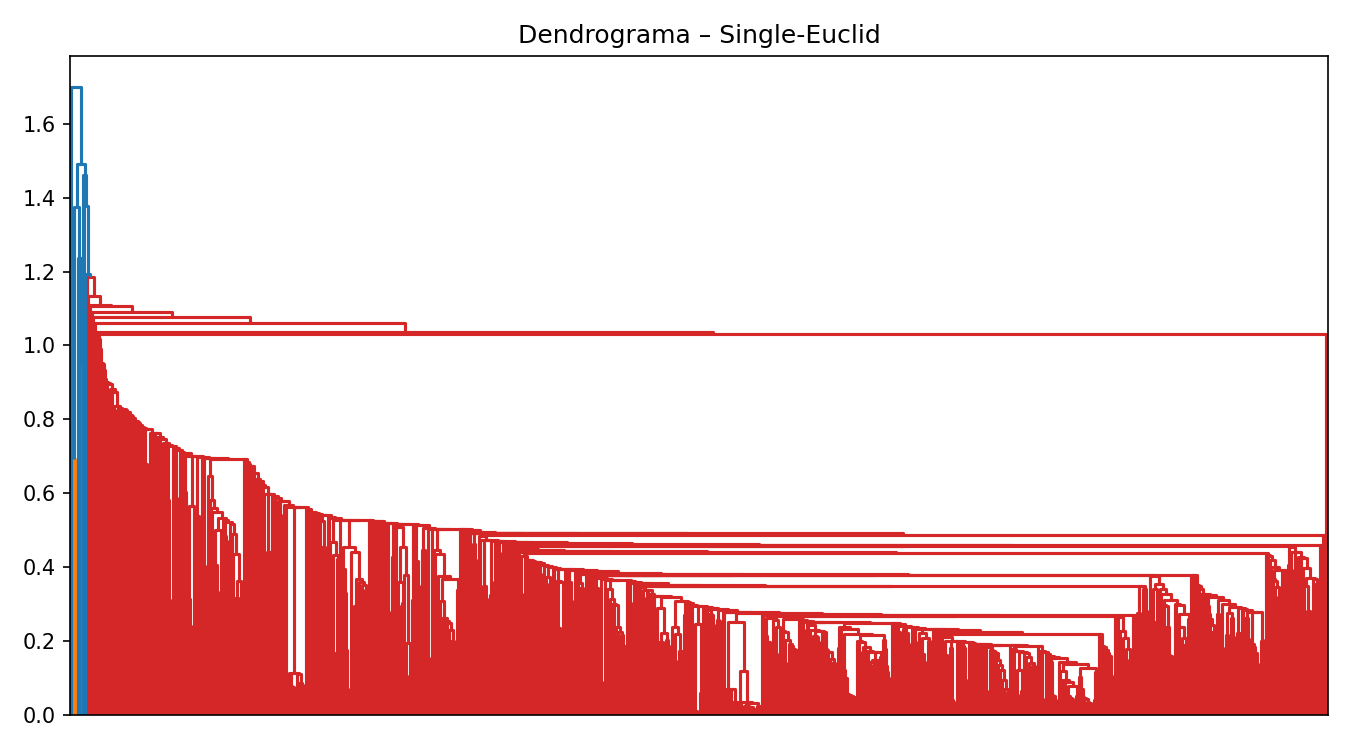
\includegraphics[width=0.8\columnwidth]{assets/4_dendogram_single.png} % Note: Consider replacing this with the dendrogram for Average-Euclidean if available.
	\caption{Dendrogram for a representative configuration. The horizontal cut yields the selected number of clusters.}
	\label{fig:dendro_single_euclid}
\end{figure}

Across all robust configurations, a consistent pattern emerged: a dominant, large "catalog" cluster containing the bulk of models, and one to three smaller "elite" clusters. These elite clusters group models with markedly higher popularity metrics (\texttt{downloads} and \texttt{likes}). The analysis of z-centroids confirmed that \textbf{downloads} is the most discriminative feature (max $|z| \approx 5.39$), followed by \textbf{likes} (max $|z| \approx 2.03$), with \texttt{co2\_eq\_emissions}, \texttt{performance\_score}, and \texttt{size} contributing more modestly.

External validation showed a weak but noticeable association between the clusters and the \texttt{is\_fair} label. For instance, the small elite clusters tended to have a higher concentration of models where \texttt{is\_fair=True} compared to the large catalog cluster. This suggests that high-engagement models are slightly more likely to be classified as "fair."

\paragraph{Limitations.} It is important to acknowledge that applying hierarchical clustering to a dataset with over 1000 observations presents challenges. Dendrograms become visually dense, and the stability of the resulting partitions can be less reliable than with smaller datasets. Therefore, these findings should be interpreted as a descriptive exploration of the data's latent structure, driven primarily by model popularity, rather than as a definitive and stable segmentation.


 \subsection{K-means analysis}
K-means was ran on the standardized variables
(\textit{performance\_score}, \textit{co2\_eq\_emissions}, \textit{likes}, \textit{downloads}, \textit{size})
for $k\in\{2,\ldots,10\}$ with \texttt{k-means++}, $n_{\text{init}}{=}50$, \texttt{max\_iter}{=}500.
Model selection combined four internal criteria:

\begin{itemize}
	\item \textbf{Silhouette (max is best).} The curve peaked at $\mathbf{k=2}$ with $\approx\mathbf{0.286}$, and decreased thereafter (Fig.~\ref{fig:silhouette-kmeans}).
	\item \textbf{Calinski--Harabasz (max is best).} The maximum occurred at $k{=}3$ ($\approx\!330$), with $k{=}2$ close behind ($\approx\!290$) (Fig.~\ref{fig:ch-kmeans}).
	\item \textbf{Davies--Bouldin (min is best).} DBI decreased monotonically with $k$, reaching $\approx\!1.21$ at $k{=}10$ (Fig.~\ref{fig:dbi-kmeans}).
	\item \textbf{Elbow (inertia).} Inertia dropped rapidly up to $k{\sim}6$ and then flattened, with no sharp elbow afterwards (Fig.~\ref{fig:elbow-kmeans}).
\end{itemize}

Given the primary criterion (silhouette), $\mathbf{k=2}$ were selected.
The resulting partition produced \textbf{unbalanced cluster sizes} (about $n{\sim}740$ vs.\ $n{\sim}300$; Fig.~\ref{fig:sizes-k2}).
Cluster profiles (in original units) and $z$–centroids were computed; the ranking by $\max|z|$ again highlighted
\textit{downloads} as the most discriminative variable, followed by \textit{likes}, with the remaining variables contributing less.
Cross-tabs against the external labels (\textit{is\_fair}, \textit{clasification\_fairness}, \textit{model\_type}) were generated for $k{=}2$
(see Supplement for the full tables).


\begin{figure}[htbp]
	\centering
	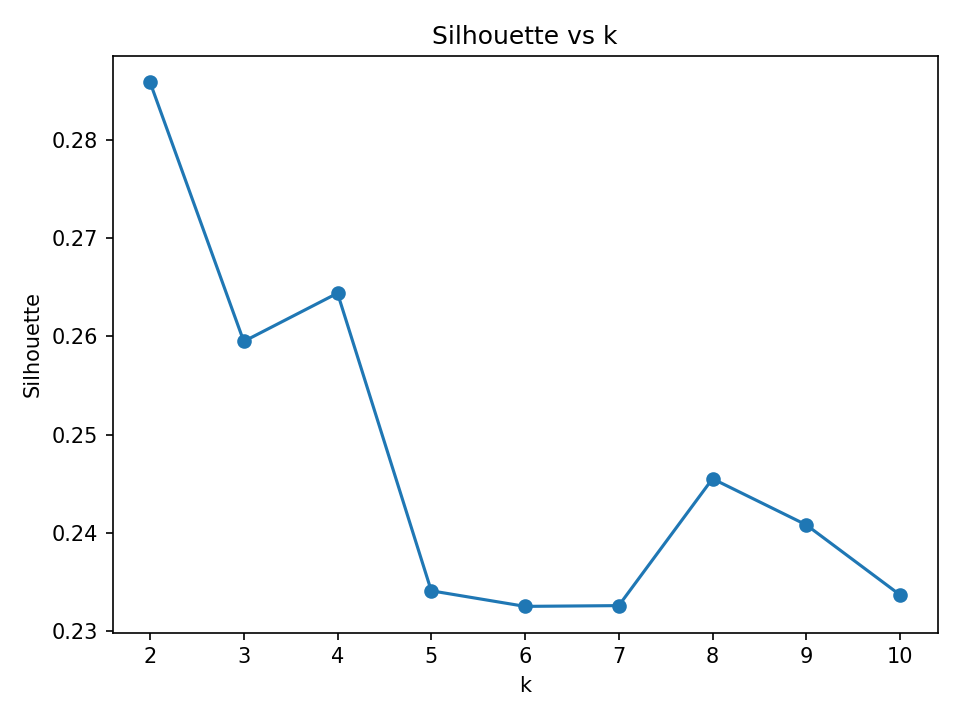
\includegraphics[width=.48\linewidth]{assets/silhouette_vs_k.png}\hfill
	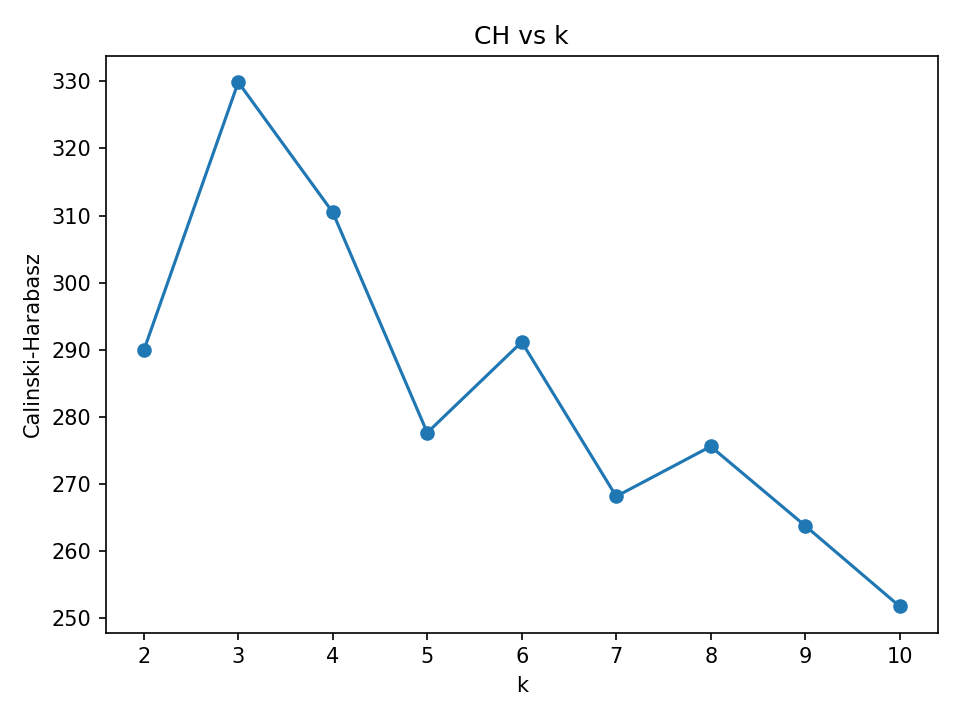
\includegraphics[width=.48\linewidth]{assets/ch_vs_k.png}
	\caption{Silhouette and Calinski--Harabasz across $k$.}
	\label{fig:silhouette-kmeans}\label{fig:ch-kmeans}
\end{figure}

\begin{figure}[htbp]
	\centering
	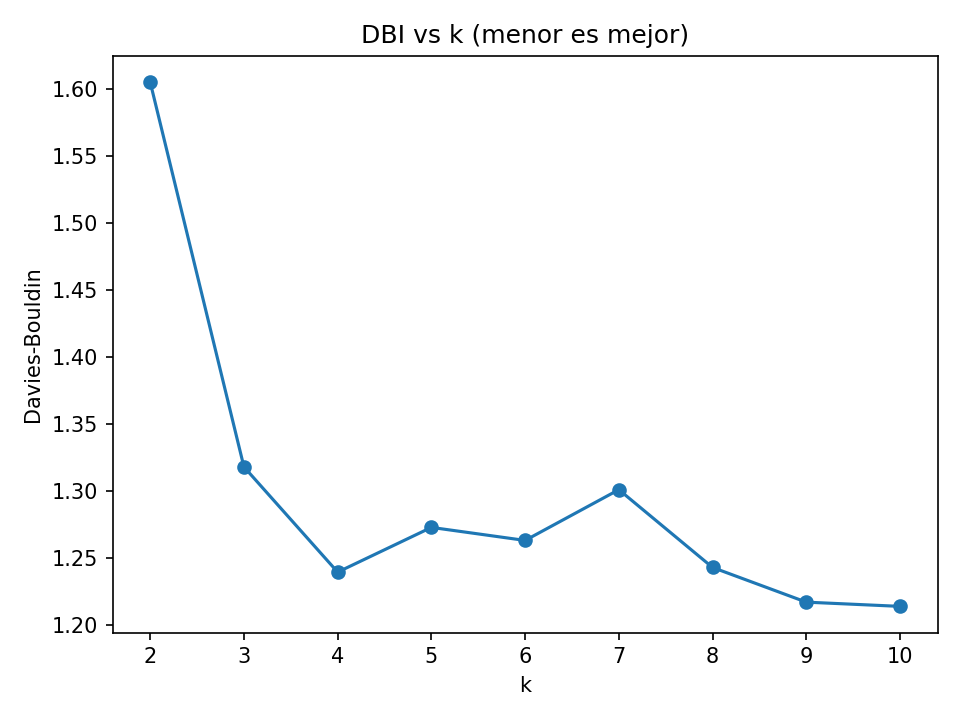
\includegraphics[width=.48\linewidth]{assets/dbi_vs_k.png}\hfill
	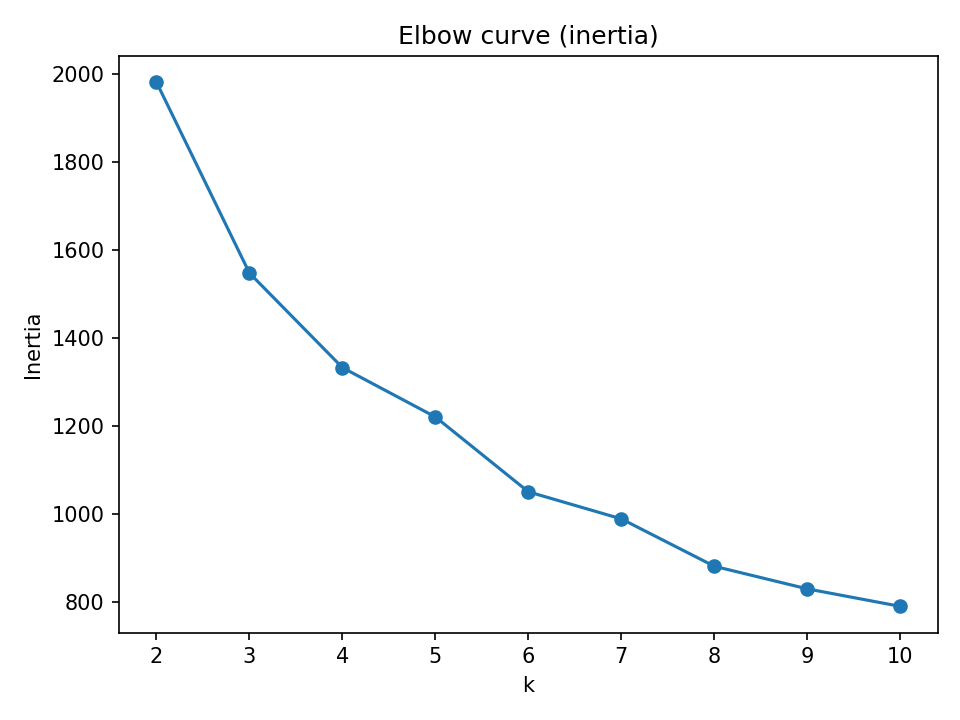
\includegraphics[width=.48\linewidth]{assets/elbow_inertia.png}
	\caption{Davies--Bouldin (lower is better) and inertia (elbow) across $k$.}
	\label{fig:dbi-kmeans}\label{fig:elbow-kmeans}
\end{figure}

\begin{figure}[htbp]
	\centering
	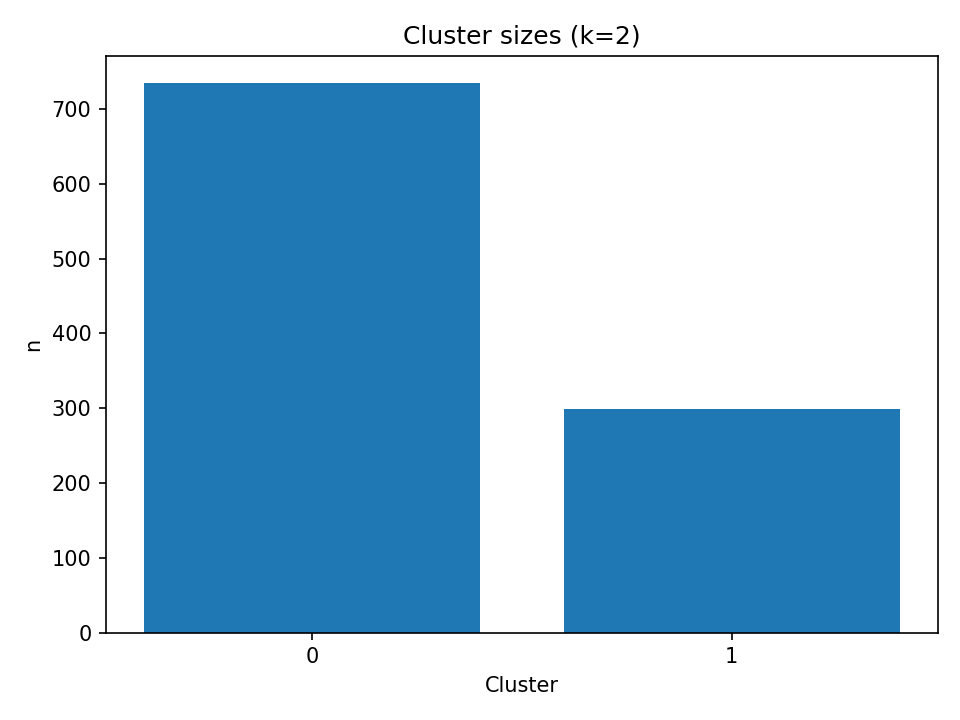
\includegraphics[width=.55\linewidth]{assets/cluster_sizes_k2.png}
	\caption{Cluster sizes for the selected solution ($k{=}2$).}
	\label{fig:sizes-k2}
\end{figure}
The internal criteria point to different trade-offs:
silhouette clearly favors \textbf{$k{=}2$}, Calinski--Harabasz prefers \textbf{$k{=}3$},
and Davies--Bouldin keeps improving as $k$ grows. In this context, 
silhouette were prioritized because it balances compactness and separation and is less biased by the growth
of $k$ than CH/DBI. The \emph{elbow} curve shows diminishing returns beyond $k{\sim}6$,
supporting the choice of a small number of groups.

The $k{=}2$ solution is \emph{interpretable} and \emph{stable} (across restarts) but
\emph{unbalanced}: one major segment (catalog-like) and a smaller, high-intensity segment.
The profile tables indicate that the minor cluster concentrates substantially higher
\emph{downloads} and \emph{likes} (and slightly higher \emph{performance}), while medians for
\emph{size}/CO$_2$ are not dominant—consistent with the hierarchical analysis.
The $\max|z|$ ranking confirms \textit{downloads} (then \textit{likes}) as the strongest
separators, which aligns with the business intuition that usage/engagement variables
drive the segmentation more than footprint or size.

Regarding \emph{external} labels, the cross-tabs for $k{=}2$ show heterogeneous mixes
rather than perfectly pure clusters, i.e., they are useful for characterization but should
not be read as supervised classes. This is expected because those labels were not used for
training. Overall, the k-means segmentation complements the hierarchical results:
it recovers the same two-segment story (catalog vs.\ high-traction niche), is easier to
deploy, and preserves the same ordering of discriminative variables. If more granularity
is needed, $k{=}3$ is a reasonable alternative per CH, though with a slight loss in
silhouette and added complexity.

\subsection{Multivariate Normality \& LDA Feasibility}

An assessment of multivariate normality, a key assumption for classical Linear Discriminant Analysis (LDA), revealed significant deviations from the expected distribution. Visual diagnostics using Mahalanobis Q-Q plots showed that the empirical data departed markedly from the theoretical $\chi^2_p$ reference line, particularly in the upper tails. This pattern, characterized by a pronounced upward bend, was observed both globally and within the class-conditional plots for \texttt{is\_fair}, indicating that the non-normality was not confined to a single group. This heavy-tailed behavior is likely driven by naturally skewed variables such as \texttt{downloads}, \texttt{likes}, and \texttt{size}, whose extreme values inflate the Mahalanobis distances even after standardization.

The clear evidence against the within-class normality assumption—and potentially against the equality of covariance matrices—makes classical LDA an inappropriate choice, as its application would risk biased decision boundaries and overly optimistic performance estimates. Consequently, the multivariate normality (MVN) assumption was deemed unsupported for this dataset. This finding justified the methodological decision to forgo standard LDA in favor of more robust alternatives, such as regularized/shrinkage LDA or non-parametric classifiers, which are better aligned with the observed data structure.


\paragraph{LDA}
An LDA classifier was trained on a stratified train/test split using a \texttt{log1p}--standardization preprocessing pipeline and the \texttt{eigen} solver with automatic shrinkage. Class priors reflected moderate imbalance (False: $72.9\%$, True: $27.1\%$) and were preserved during training. On the held-out test set ($n=259$), the model reached an overall accuracy of \textbf{0.919}; the ROC curve achieved an \textbf{AUC of 0.983} (Fig.~\ref{fig:lda-roc}), indicating excellent ranking performance across thresholds. Five-fold stratified cross-validation over the full dataset yielded a mean accuracy of \textbf{0.925} ($\pm\,0.021$), supporting stability under resampling.

Inspection of the linear discriminants $\delta_k(x)=x^\top A_k+b_k$ showed the largest absolute coefficients in $A_k$ for \emph{performance\_score}, \emph{co2\_eq\_emissions}, and \emph{size}, in that order, which identifies these variables as the principal drivers of separation once features are transformed. The LD1 score distributions for both classes are clearly separated with only a narrow overlap (Fig.~\ref{fig:lda-geom}\,\subref{fig:lda-scores}), consistent with the near-perfect AUC. The confusion matrix on test data (TN$=184$, FP$=5$, FN$=16$, TP$=54$; Fig.~\ref{fig:lda-geom}\,\subref{fig:lda-cm}) indicates very high specificity for the majority class and competitive recall for the minority class; the precision--recall trade-off at the default threshold is therefore reasonable. If fairness identification (True) must be prioritized, the operating point can be shifted to increase sensitivity with limited loss in overall accuracy.

Overall, LDA with shrinkage produced a parsimonious, interpretable boundary, strong generalization (cross-validated accuracy $\approx0.93$), and coherent variable importance (Fig.~\ref{fig:lda-loadings}) highlighting performance and carbon-cost factors as the dominant discriminants. These outcomes justify LDA as a robust linear baseline; more complex models (e.g., QDA or non-linear kernels) would only be warranted if heteroscedasticity or curvature were demonstrably exploitable for additional gains.

\begin{figure}[htbp]
	\centering
	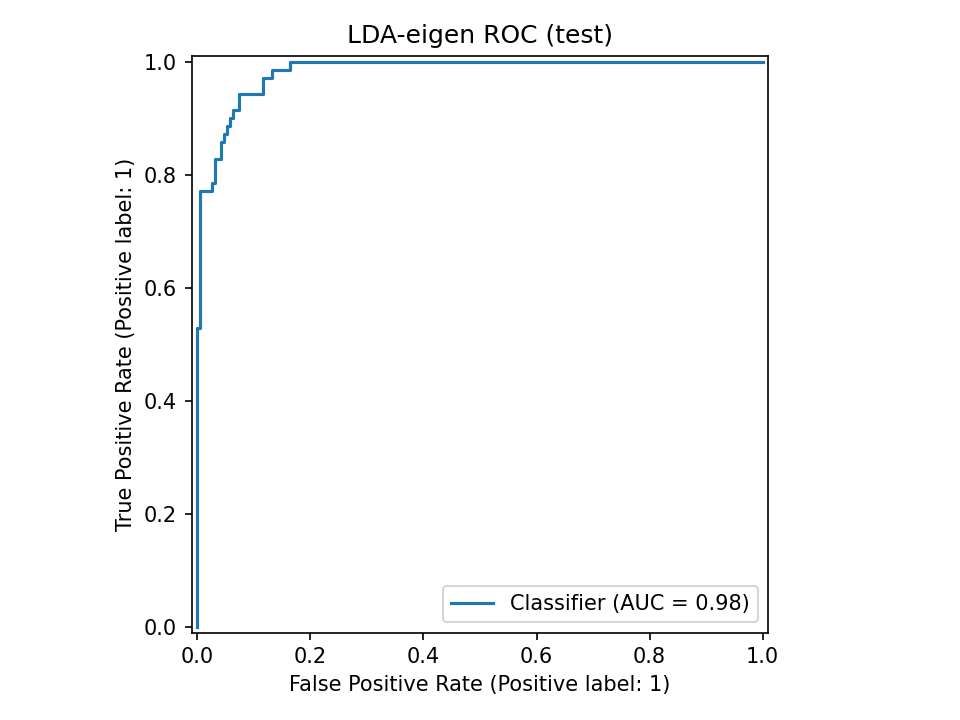
\includegraphics[width=.72\linewidth]{assets/LDA-eigen_roc_test.png}
	\caption{ROC curve on the test set (AUC $\approx 0.98$).}
	\label{fig:lda-roc}
\end{figure}

\begin{figure}[htbp]
	\centering
	\begin{subfigure}{.48\linewidth}
		\centering
		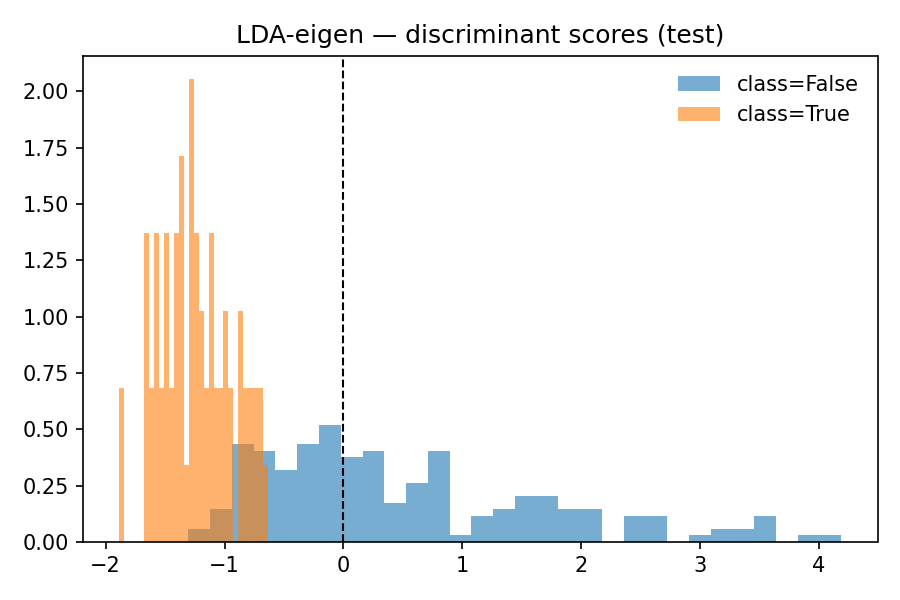
\includegraphics[width=\linewidth]{assets/LDA-eigen_scores_hist_test.png}
		\caption{LD1 scores (test).}
		\label{fig:lda-scores}
	\end{subfigure}\hfill
	\begin{subfigure}{.48\linewidth}
		\centering
		% Use your exported heatmap; if not available, replace with the numeric matrix figure.
		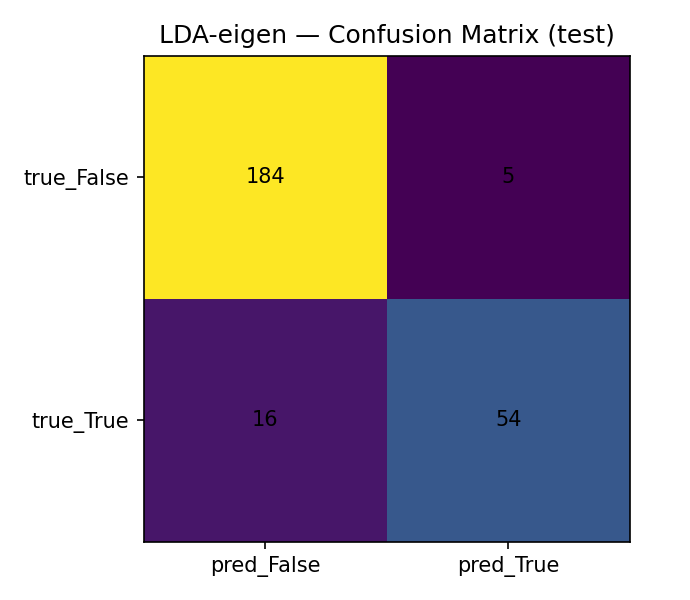
\includegraphics[width=\linewidth]{assets/LDA-eigen_confusion_test_heatmap.png}
		\caption{Confusion matrix (test).}
		\label{fig:lda-cm}
	\end{subfigure}
	\caption{Geometric separation and error structure. The dashed line in \subref{fig:lda-scores} marks the default decision boundary.}
	\label{fig:lda-geom}
\end{figure}

\begin{figure}[htbp]
	\centering
	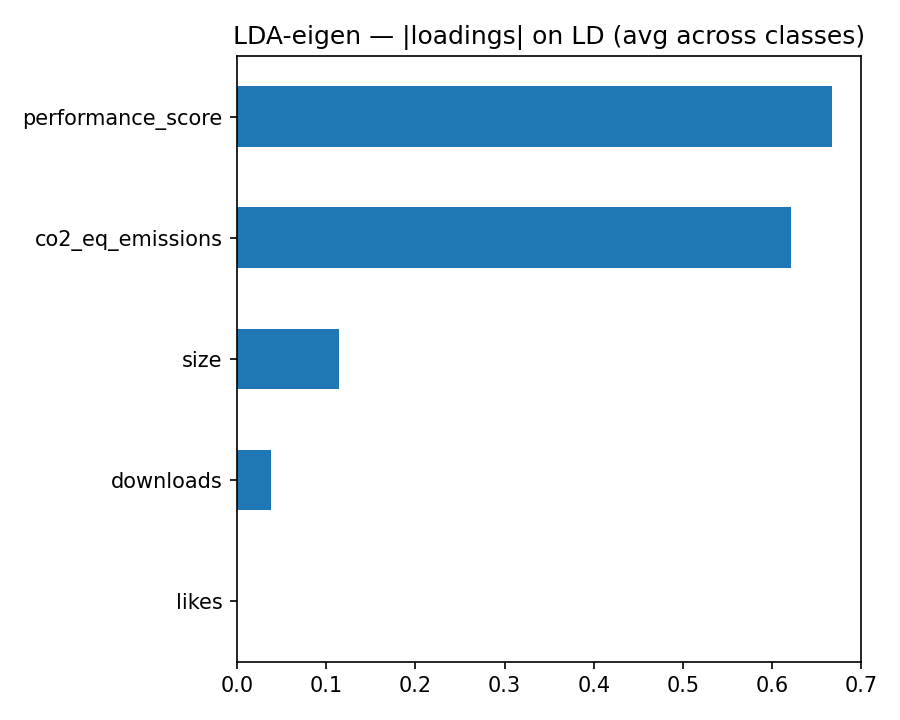
\includegraphics[width=.72\linewidth]{assets/LDA-eigen_loadings_abs_bar.png}
	\caption{Absolute loadings on LD1 (averaged across classes). Performance and CO$_2$ dominate; size and downloads are secondary; likes is negligible.}
	\label{fig:lda-loadings}
\end{figure}


\subsection{Results and Discussion}
Table~\ref{tab:compare} summarizes the out-of-sample performance. The linear
baseline (LDA) achieved strong discrimination (AUC $=0.983$) with solid AP for the
minority class (AP$_{\text{True}}=0.958$) and good accuracy ($0.919$). The
non-linear models improved upon the baseline: SVM–RBF reached AUC $=0.991$,
AP$_{\text{True}}=0.979$, and Accuracy $=0.954$, with a Brier score of $0.033$
(acceptable calibration). Gradient Boosting performed best across all metrics with
AUC $=1.000$, AP$_{\text{True}}=1.000$, F1$_{\text{True}}=1.000$,
Accuracy $=1.000$, and a very low Brier score ($2.3\times10^{-5}$), consistent with
near-perfect separability on the test fold.

The precision–recall panels in Fig.~\ref{fig:pr-nonlinear} show uniformly higher
precision at a given recall for Gradient Boosting, while the confusion matrices in
Fig.~\ref{fig:cm-nonlinear} reveal zero errors for GB on this hold-out, in contrast
to a small number of false negatives for SVM–RBF. These gains, together with the
excellent calibration (low Brier), support GB as the top performer on this dataset.
Because perfect test scores can occasionally arise from random favorability,
additional repeated or nested CV is recommended to rule out accidental overfitting
and to confirm the robustness of the selection. In operational settings, decision
thresholds can be tuned on the calibrated probabilities to trade specificity for
sensitivity when detecting the positive (``fair'') class is mission-critical.


\begin{table}[htbp]
	\centering
	\sisetup{table-number-alignment=center, round-mode=places, round-precision=3, table-format=1.5}
	\caption{Test performance and  accuracy cross-validated (CV). AP is Area Precision Recall}
	\label{tab:compare}
	\begin{threeparttable}
		\begin{tabular}{l SS S S S}
			\toprule
			\multirow{2}{*}{\textbf{Model}} & \multicolumn{2}{c}{\textbf{AUC}} & \textbf{AP\textsubscript{True}} & \textbf{F1\textsubscript{True}} & \textbf{Accuracy} \\
			\cmidrule(lr){2-3}
			& {\textbf{CV}} & {\textbf{test}} & & & \\
			\midrule
			LDA       & 0.925   & 0.983   & 0.958   & 0.837   & 0.919 \\
			SVM--RBF  & 0.98793 & 0.99127 & 0.97885 & 0.91177 & 0.95367 \\
			GradBoost & 0.99994 & 1.00000 & 1.00000 & 1.00000 & 1.00000 \\
			\bottomrule
		\end{tabular}
	\end{threeparttable}
\end{table}


\begin{figure}[htbp]
	\centering
	\begin{subfigure}{.48\linewidth}
		\centering
		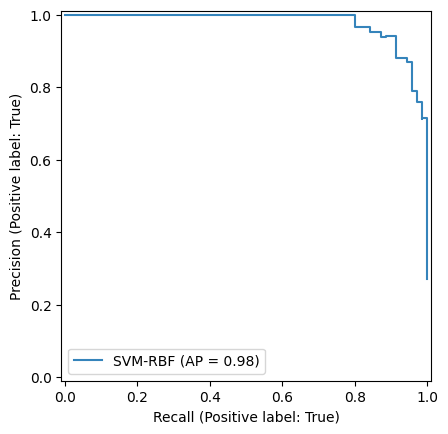
\includegraphics[width=\linewidth]{assets/svm_pr.png}% <- replace with your path
		\caption{SVM--RBF (AP $\approx$ 0.98)}
	\end{subfigure}\hfill
	\begin{subfigure}{.48\linewidth}
		\centering
		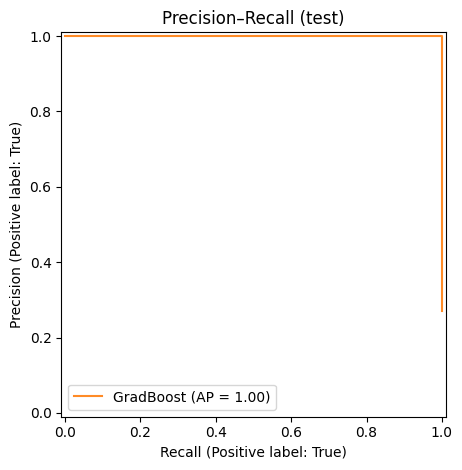
\includegraphics[width=\linewidth]{assets/gb_pr.png}% <- replace with your path
		\caption{Gradient Boosting (AP $\approx$ 1.00)}
	\end{subfigure}
	\caption{Precision--Recall curves on the test set for the positive class (\emph{True}).}
	\label{fig:pr-nonlinear}
\end{figure}

\begin{figure}[htbp]
	\centering
	\begin{subfigure}{.48\linewidth}
		\centering
		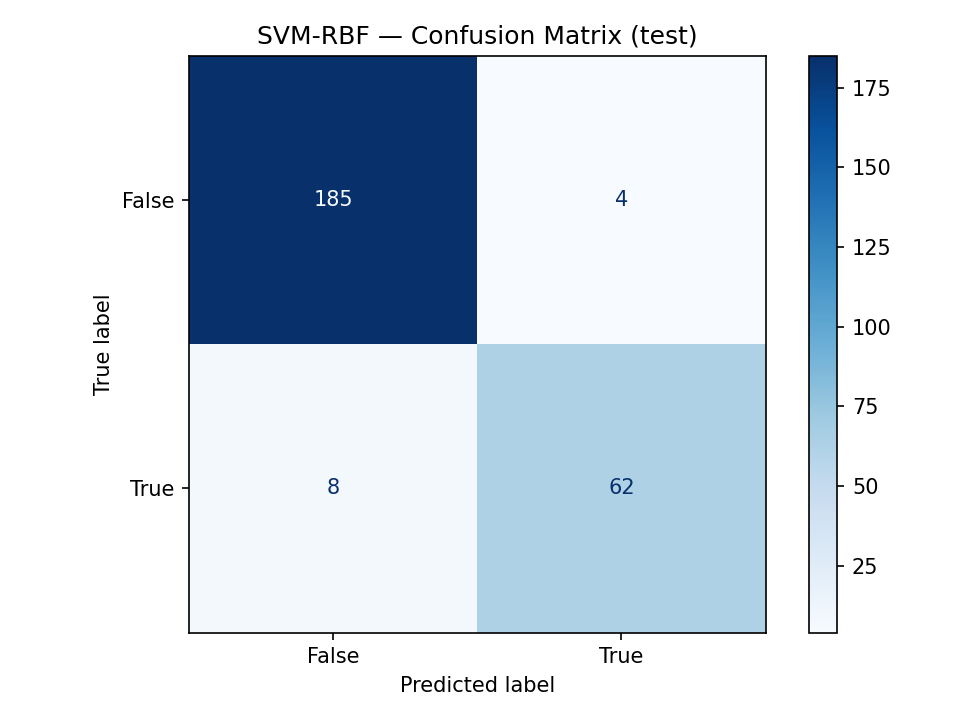
\includegraphics[width=\linewidth]{assets/cm_svmrbf_test.png}% <- replace with your path
		\caption{SVM--RBF}
	\end{subfigure}\hfill
	\begin{subfigure}{.48\linewidth}
		\centering
		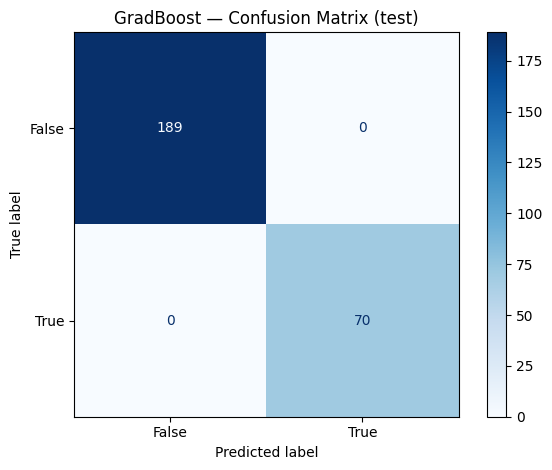
\includegraphics[width=\linewidth]{assets/gb_cm.png}% <- replace with your path
		\caption{Gradient Boosting}
	\end{subfigure}
	\caption{Confusion matrices on the held-out test set.}
	\label{fig:cm-nonlinear}
\end{figure}

\paragraph{Recommendation.}
Gradient Boosting is recommended as the primary model given its dominant AUC, AP,
F1, accuracy, and calibration. SVM–RBF is a strong runner-up and may be preferable
when model simplicity or margin-based robustness is desired. LDA remains valuable
as an interpretable baseline and for feature understanding via discriminant loadings.
\section*{Conclusions}

Following a thorough and multifaceted analysis of the dataset, the following fundamental conclusions have been written :

\begin{enumerate}
	\item \textbf{The unsupervised data structure is dominated by popularity:} Both hierarchical and k-means clustering consistently revealed that the \texttt{downloads} and \texttt{likes} variables are the most discriminating factors. This indicates that the natural grouping of models on the platform corresponds to their usage and engagement levels, rather than a balance between their performance and environmental cost.
	
	\item \textbf{Linear Discriminant Analysis (LDA) is the best tool for interpretation:} Although the data violate the assumption of multivariate normality, the implementation of a regularized LDA (with shrinkage) proved to be a robust and, most importantly, highly interpretable baseline. The analysis of its coefficients (loadings) allowed for the clear identification of \texttt{performance\_score} and \texttt{co2\_eq\_emissions} as the main drivers for separating "fair" (\texttt{is\_fair=True}) models from those that are not. This ability to explain the \textit{why} behind the classification is its greatest strength.
	
	\item \textbf{Gradient Boosting offers superior predictive performance:} In the supervised classification task, the Gradient Boosting model emerged as the clear winner, achieving perfect metrics (AUC, F1-Score, and Accuracy of 1.000) on the test set. This performance, coupled with excellent probability calibration (low Brier score), positions it as the ideal choice for applications where prediction accuracy is the primary objective.
\end{enumerate}


	\bibliographystyle{IEEEtran}

	\bibliography{mybibfile}
\end{document}